\documentclass{article}
\usepackage{../repsty}
\usepackage{threeparttable}
\usepackage{url}
\usepackage{hyperref}
\newcommand{\Dim}[1]{\mathrm{#1}}




\begin{document}

\title{Statistical modeling}
\maketitle

\section*{Introduction}
\dots
Since the estimate $\Ayy*$ is obtained as a difference statistic of the slopes in the up- and down-polarized trials, its variance $\SE{\Ayy*} = C\sqrt{2}\cdot\SE{\slp*}$, with the proportionality coefficient (see Table~\ref{tbl:Param}) $C = (\nu\CS[0]\Thick P^t\DP)^{-1} \approx 1.3\cdot 10^{5}$. 

For the mean, 
\begin{equation}\label{eq:AvgAyySE}
	\SE{\avg{\Ayy*}} = \frac{\SE{\Ayy*}}{\sqrt N} = \sqrt{2}\sqrt{\frac hH}\cdot\SE{\Ayy*},
\end{equation}
where $H$ is the beam time, $h$ the cycle length, and so the number of estimate pairs $N = \sfrac{H}{2h}$.

\begin{table}
\centering
\caption{Parameter values (June 2016)\label{tbl:Param}}
\begin{threeparttable}[h]
\begin{tabular}{llr}
\hline\hline
Parameter					& Value 				& Dimension \\
\hline
$\nu$						& 0.79 					& MHz \\
$\Thick$					& $1.1\cdot 10^{14}$	& $\Dim{at\cdot cm^{-2}}$ \\
$P^t$						& 0.88					& -- \\
$\DP$						& 1.48					& -- \\
$\CS[0]$\tnote{a}			& 70					& mb\\
\hline
\end{tabular}
\begin{tablenotes}
	\item[a]{From Particle Data Grpoup \url{http://pdg.lbl.gov/2016/hadronic-xsections/rpp2014-pd_pn_plots.pdf}}
\end{tablenotes}
\end{threeparttable}
\end{table}



\section{Required beam time}
\newcommand{\Tint}{\Delta t}
\DeclareDocumentCommand{\v}{O{}mo}{\sigma^2_{#1}\bkt*{#2\IfValueT{#3}{|~ #3}}}

Under the Gauss-Markov conditions, the slope estimate's standard error is
\begin{equation}\label{eq:SlpVarGM}
	\SE{\slp*} = \frac{\SE{\err}}{\sqrt{\sum_k (t_k - \avg{t})^2}},
\end{equation}
where $\SE{\err}$ is the measurement resolution.

Since the measurements are taken uniformly in time with the step $\Tint$, rewriting eq.~\eqref{eq:SlpVarGM} in physical terms gets:
\begin{align*}
	\sum_{k=1}^K (t_k - \avg{t})^2 &= \sum_k (k\Tint - \frac{1}{K}\sum_{k=1}^K k\Tint)^2; \\
	\frac{1}{K}\sum_{k=1}^K k\Tint  &= \frac{\Tint}{2}(K+1)\equiv \Tint\mu, \\
	\sum_k (k\Tint - \mu\Tint)^2 	&= \Tint^2\sum_k\bkt{
											k^2 - 2k\mu + \mu^2
										} \\
									&= \Tint^2\bkt{\sum_k k^2 - 2\mu\sum_k k + \mu^2K} \\
									&= \Tint^2\bkt{
											\frac{2K+1}{3}K\mu - 2\mu^2K + \mu^2K
										} 
		 							 = \Tint^2\mu K\bkt{\frac{2K+1}{3} - \mu} \\
									&= \Tint^2\mu K \frac{K-1}{6} \\
									&= \frac{\Tint^2}{12}K(K^2-1),
\shortintertext{and hence}									
	\sqrt{\sum_{k=1}^K(t_k - \avg{t})^2} = \frac{\Tint}{2\sqrt{3}}\sqrt{K}\sqrt{K^2-1}.
\end{align*}
As the number of measurements grows, $K \gg 1$, $K^2-1\approx K^2$, and so
\[
	\sqrt{\sum_k (t_k - \avg{T})^2} \approx \frac{\Tint}{2\sqrt{3}}K\sqrt{K}.
\]

The number $K$ of measurements that go into evaluating a slope is related to the state time $h$ as $K\Tint = h$, hence
\[
	\sqrt{\sum_{k=1}^K (t_k - \avg{t})^2} \approx \frac{h\sqrt{h}}{2\sqrt{3}\sqrt{\Tint}}.
\]
Finally, for the slope variance,
\begin{equation}\label{eq:SlpVar}
	\SE{\slp*} = 2\sqrt{3}\sqrt{\frac{\Delta t}{h}}\frac{\SE{\err}}{h}.
\end{equation}

By plugging it in eq.~\eqref{eq:AvgAyySE} we get
\begin{equation}\label{eq:AvgAyySEPhys}
\SE{\avg{\Ayy*}} = 4\sqrt{3}C\cdot \frac{\sqrt{\Tint}}{h\sqrt{H}}\cdot\SE{\err}.
\end{equation}
The estimated beam time for different values of measurement resolution and precision, computed for the case of 15-minute cycles, is shown in Figure~\ref{fig:BeamTime}.

\begin{figure}[h]
\centering
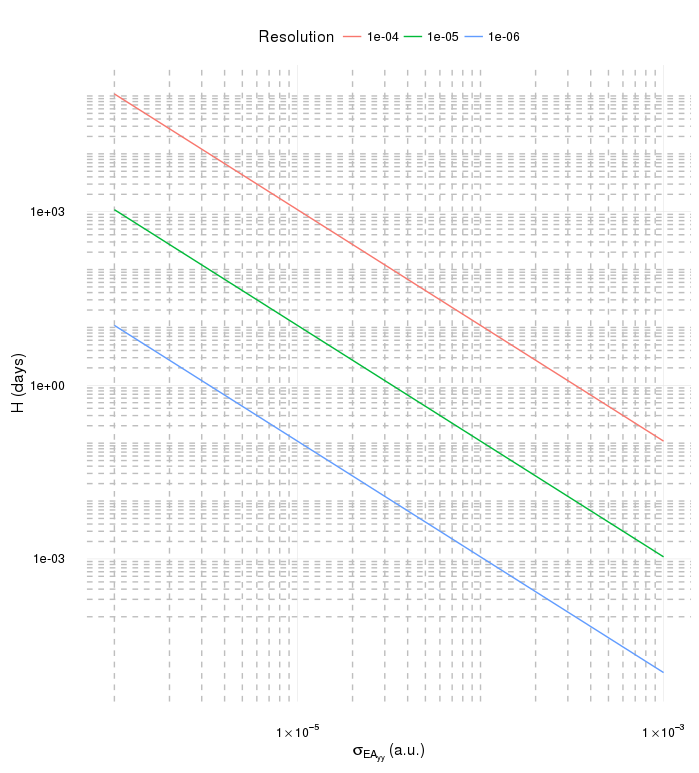
\includegraphics[scale=1]{BeamTime_15minCycle}
\caption{Beam time (in full days) as a function of the standard error of the mean $\Ayy$ estimate, required in the case of 15-minute cycles.\label{fig:BeamTime}}
\end{figure}

\section{Appropriate cycle length}
\DeclareDocumentCommand{\Xpct}{O{}mo}{\mathrm{E}_{#1}\bkt*{#2\IfValueT{#3}{|~ #3}}}
Suppose the slope varies; in that case the law of total variance says that 
\begin{equation}\label{eq:VarSlpLTV}
	\v{\slp*} = \Xpct[\slp]{\v{\slp*}[\slp]} + \v[\slp]{\Xpct{\slp*}[\slp]}.
\end{equation}
\begin{align*}
\Xpct{\slp*}[\slp] 	&= \slp, \\
\v{\slp*}[\slp] 	&= 12\frac{\Tint}{h}\frac{\v{\err}}{h^2}, \tag{eq.~\eqref{eq:SlpVar}}
\shortintertext{and hence}
\v{\avg{\Ayy*}}		&= \frac{4 C^2}{H}\bkt{12\Tint\cdot\frac{\v{\err}}{h^2} + h\cdot\v{\slp}}.
\end{align*}
The first term describes the estimate's statistical precision, the second its accuracy. By decreasing the cycle length we reduce precision, but improve accuracy. The accuracy is improved simply by virtue of better averaging of $\v{\slp}$.

From the last expression, the best variance is achieved at
\begin{equation}
	h_{best} = \sqrt[3]{24\cdot \Tint} \bkt{\frac{\v{\err}}{\v{\slp}}}^{1/3}.
\end{equation}

\begin{table}
\centering
\begin{tabular}{lrr}
\hline\hline
$\SE{\err}$			&	$h_{best}$ (min)	& $\SE{\avg{\Ayy*}}$\\
\hline
$5\cdot10^{-3}$		&	141					& $8\cdot10^{-4}$\\
$1\cdot10^{-3}$		&	48					& $3\cdot10^{-4}$\\
$5\cdot10^{-4}$		&	30					& $3\cdot10^{-4}$\\
$1\cdot10^{-4}$		&	10					& $2\cdot10^{-4}$\\
$5\cdot10^{-5}$		&	7					& $1\cdot10^{-4}$\\
\end{tabular}
\end{table}

\begin{figure}
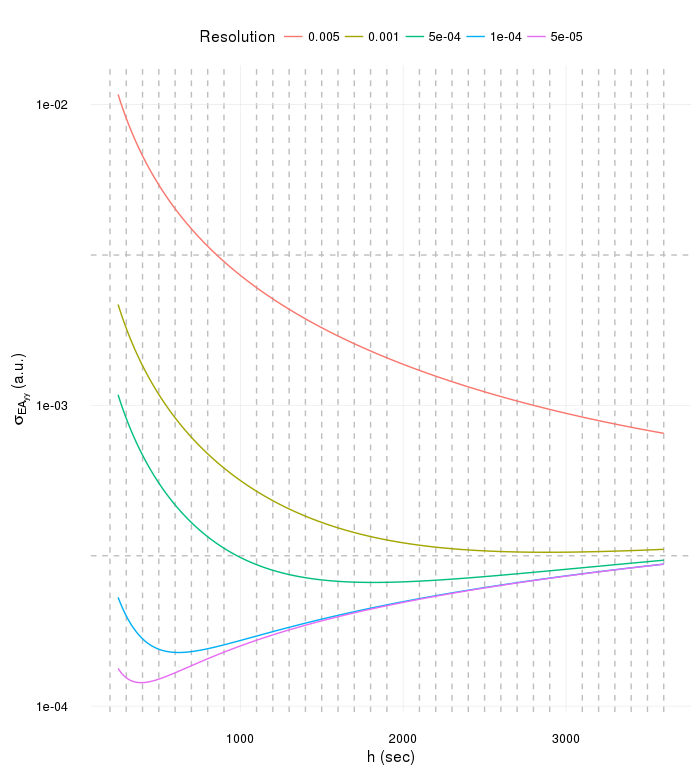
\includegraphics[scale=1]{AyySE_varb_15}
\caption{The standard error of the mean $\Ayy$ estimate as a function of cycle length when the inherent slope variation $\v{\slp} = 1\cdot10^{-15}$.}
\end{figure}

\end{document}